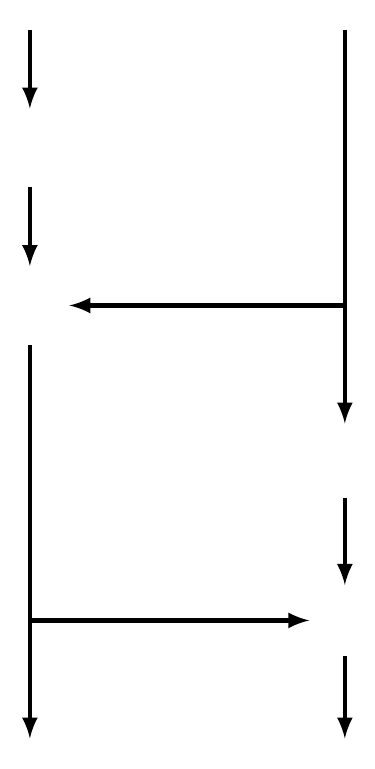
\begin{tikzpicture}[ultra thick,>=latex]
% Reference grid (temporary)
%\draw[help lines] (0,0) grid (16,16);

% Inputs A and B
\drawMixerInputs
\draw[->] (1,15) to (1,14);
\draw[->] (5,15) to (5,10);

% Rotation
\drawRot{1}{13.5}

% Modular addition
\drawAdder{0.5}{12}

% Adder inputs
\draw[->] (1,13) to (1,12);
\draw[->] (5,11.5) to (1.5,11.5);

% Rotation
\drawRot{5}{9.5}

% XOR
\drawXOR{5}{7.5}

% XOR inputs
\draw[->] (1,7.5) to (4.55,7.5);
\draw[->] (5,9.05) to (5,7.95);

% Outputs A' and B'
\draw[->] (1,11) to (1,6);
\draw[->] (5,7.05) to (5,6);
\drawMixerOutputs{10}

\end{tikzpicture}
